\documentclass[../thesis.tex]{subfiles}
% Separate preamble for this subfile. This preamble is loaded last, so one can override various functions before \begin{document}

% Better comment extension for Vscode colors these comments differently
% Normal comment color
% * Important information
% ! ALERT
% ? Question
% TODO stuff to do
% // This is strikethrough


\begin{document}

\mycomment{

Den tiden som gjennstår:


Jo høyere dimensjon vi får jo mer eksotisk kan disse tilingene bli. Står noe referanser til i paperet. 
Keller hadde en teori om at enhver tiling må være av den typen -- (Se for deg enhetskuben i 2D)
enhver tiling nødvendigvis medføre at,
alle tiles har en full felles kant med en annen tile

i 2D gjelder det her med at man har to kanter hvor man har en full felles kant (med den over og den under)


i 1D har man ingen sidekant, det er et punkt
men poenget er at i veldig høye dimensjoner så kan tilingene bli mer eksotiske, og et utrykk for det er at du ikke trenger å ha en full kant med noen som helst annen tile
dimensjon > 7
}




%!  Uformell definisjon av hva vi mener med det
%* Figurer og eksempler, 1 eller 2D, trenger ikke gå opp til 3D.
%* Det må inn noen figurer som gjør at når det kommer til tilings, så finnes det noen mengder som bare tiler med translasjoner, og noen mengder som vil krevet at man roterer eller speiling, og at vi skal holde oss til de som er kun med translasjon.

Informally, to tile refers to the process of covering some surface with objects. These objects are called tiles and come in a variety of shapes and sizes. When we are tiling, we essentially place copies of the tile next to each other in a systematic way, intending to leave no gaps and no overlaps between the tiles. The resulting tiling can be as simple as the one shown in \cref{fig:tiling_one} where we have used a single tile, the unit square, to tile the plane, or as complex as \cref{fig:tiling_two} where we have used four different tiles to tile the plane. The first is an example of what is known as a \emph{monohedral tiling} in which all tiles are congruent \cite[p. 20]{grunbaumTilingsPatterns1987}, and the latter is an example of a Penrose tiling which are well known for being non-periodic \cite{penrosePentaplexityClassNonPeriodic1979}. %* PAge 535 har også penrose tilings
% non-periodic tiling, meaning that there is no period paralellogram \SigridChange{KORT FORTALT}. 





\begin{figure}[h!]%h!
    \centering
    \begin{subfigure}{.47\textwidth}
        \centering
        %\includegraphics[width=0.9\linewidth]{spec_no_shift.jpg}
        %* Figure 1
        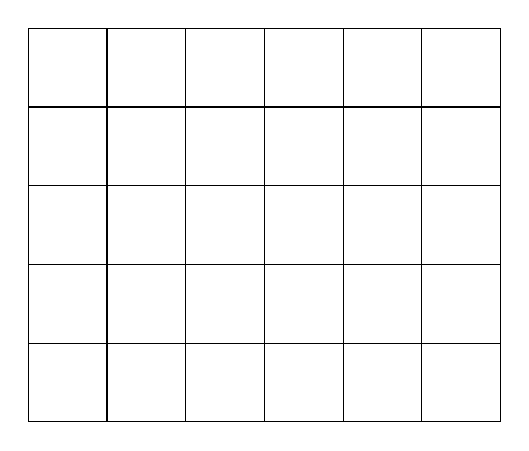
\begin{tikzpicture}[scale=1]
            % Define the tile
            \def\tile{
              % Draw the unit square
              \draw (0,0) rectangle (1,1);
            }
          
            % Draw the tiling pattern
            \foreach \x in {0,1,2,3,4,5}{
              \foreach \y in {0,1,2,3,4}{
                \pgfmathsetmacro{\shiftX}{\x} % Set horizontal shift
                \pgfmathsetmacro{\shiftY}{\y} % Set vertical shift
                \begin{scope}[shift={(\shiftX,\shiftY)}]
                  \tile % Draw the tile
                \end{scope}
              }
            }
        \end{tikzpicture}
        %* —————————————————
        \caption{Lattice spectra}
        \label{fig:tiling_one}
    \end{subfigure}\quad
    \begin{subfigure}{.47\textwidth}
        \centering
        \includegraphics[width=0.9\linewidth]{Penrose_Tiling_.png}
        \caption{P1 Penrose Tiling}
        \label{fig:tiling_two}
    \end{subfigure}
    \caption{Penrose original aperiodic tiling \cite{penrosePentaplexityClassNonPeriodic1979}, from \cite{inductiveloadP1TilingUsing}, forklare fargelegginen, \SigridComment{By Inductiveload - Own work, Public Domain, https://commons.wikimedia.org/w/index.php?curid=5839133}}
    \label{fig:tilingsss}
\end{figure}


Another interesting monohedral tiling 
\SigridChange{rotation and reflections}
%  https://www.wikiart.org/en/m-c-escher/flying-fish    
%  https://www.wikiart.org/en/m-c-escher/lizard-1}

\begin{figure}[t]%h!
    \centering
    \includegraphics[width=0.4\linewidth]{lizard-1.jpg}
    \caption{Lizard from \cite{m.c.escherLizard1942}}
    \label{fig:tiling_three}
\end{figure}


\mycomment{  %! Block comment
\begin{figure}[t]%h!
    \centering
    \begin{subfigure}{.47\textwidth}
        \centering
        \includegraphics[width=0.9\linewidth]{lizard-1.jpg}
        \caption{Lizard}
        %\label{fig:tiling_three}
    \end{subfigure}\quad
    \begin{subfigure}{.47\textwidth}
        \centering
        \includegraphics[width=0.9\linewidth]{flying-fish.jpg}
        \caption{Flying fish}
        \label{fig:tiling_four}
    \end{subfigure}
    \caption{from \cite{m.c.escherLizard1942}}
    \label{fig:tilingsss_two}
\end{figure}
}


However interesting the Penrose and Escher tilings are, we will only consider tilings of $\R^d$ by translation and using only the unit cube as our tile. Considering only cube-tilings might seem simple initially, but we will see that as we increase the dimension, we get increased flexibility and more complex tilings. This is especially true in higher dimensions, where highly exotic and counter-intuitive tilings exist compared to fundamental/straightforward/simple/basic lattice tilings \cite{iosevichSpectralTilingProperties1998}. One indicator of this characteristic follows/ from Keller's conjecture \cite{ott-heinrichkellerUberLuckenloseErfullung1930}. 

\begin{conjecture}
    All tilings of $\R^d$ by translations of the unit cube contain two cubes that share an entire $(d-1)$-dimensional face.
\end{conjecture}
If the dimension is two, the squares share a line; if the dimension is three, they share a face. This conjecture is now known to be true for all $d\leq 7$ after it was recently proven true in dimension seven \cite{brakensiekResolutionKellerConjecture2020}. 
% and we can still have quite the exotic and counter-intuitive tiling. %Worth emphasizing is the fact that we lack a method for determining whether a tile is the prototile of a monohedral tiling 


To begin, given a subset $\Omega$ of $\R^d$ and a discrete set $\Lambda$ of $\R^d$, we denote by $T(\Lambda)$ the set of translates 
\begin{equation*}
    T(\Lambda) = \braq{\Omega+\lambda : \lambda\in \Lambda},
\end{equation*}
where $\Omega + \lambda$ is the translate of $\Omega$ by the vector $\lambda$. That is the set
\begin{equation*}
    \Omega + \lambda = \braq{\omega + \lambda : \omega \in \Omega}.
\end{equation*}
Rather than defining tiling in terms of non-overlapping and covering of the space, we will instead define tiling in the Fourier domain, using little of our geometric intuition \cite{kolountzakisTilingsTranslation2010} \cite{kolountzakisStudyTranslationalTiling2003}. 

\begin{definition}[Tiling set]
    Let $\Omega \subset \R^d$ be a subset with nonzero measure, and consider a set $\Lambda \subset \R^d$. If
    \begin{equation}\label{eq:tiling_set}
        \sum_{\lambda \in \Lambda} \indicator{\Omega}{x-\lambda} = 1 \text{\space} a.e , \quad x \in \R^d,
    \end{equation}
    then $\Omega$ is called a \emph{tile}, and $\Lambda$ is called a \emph{tiling set} for $\Omega$. We say that $(\Omega, \Lambda)$ is a \emph{tiling pair}.
\end{definition}

%In other words, the shifts $\Omega + \lambda$ constitute a \emph{measuredisjoint covering} of $\R^d$, and we can say that $\Omega$ \emph{tile $\R^d$ by translation}, or that $\Omega$ is a \emph{tiling} of $\R^d$. 
With other words, we can also say that $\Omega$ \emph{tile $\R^d$ by translation}, or that $\Omega$ is a \emph{tiling} of $\R^d$. 

\SigridComment{INTRO  Keller}

%* Viktig, må inn en bit her om 
%* som en konsekvens av Kellers theorem så får vi nå akkurat den samme formen på disse tilings settene 
%* de må ligge inneholt i akkurat de samme typene mengder, og de kan ikke være ekte mindre for da får vi ikke oppfylt tiling kravet mitt.


% Following result shows that any tiling set for the cube is orthogonal. It is a critical step in our proof that any tiling set for the cube must be a spectrum for the cube and should be compared with the spectral version of Keller's theorem. 

%\begin{theorem}\label{thrm:keller_tiling} %* Orginale keller fra paperet
%    Given a discrete subset $T\subset \R^d$. If $T$ is a tiling set for $\Omega$, then given any pair $\lambda, \lambda' \in T$ such that $\lambda\neq\lambda'$, there exists a $j\in \braq{1,\dots,d}$ so that $\bral{t_j -t_j' } \in \N$
%\end{theorem}
\begin{theorem}[Keller's Theorem]\label{thrm:keller_tiling}
    Given a discrete subset $\Lambda \subset \R^d$. If $\Lambda$ is a tiling set for $\Omega$, then given any pair $\lambda, \lambda' \in \Lambda$ such that $\lambda\neq\lambda'$, there exists a $j\in \braq{1,\dots,d}$ so that $\lambda_j -\lambda_j' \in \intnozero$
\end{theorem}


example/lemma

In dimension one, the unit cube is simply the unit interval $I=\bras{0,1}$. 

\begin{lemma}\label{lem:tiling_unit_1d}
    The set of translates $T\brac{\Lambda}$ for $\Lambda = \Z +\alpha$ for some value $\alpha\in \R$ constitutes a tiling set for the unit cube.
\end{lemma}
%\begin{theorem}  %* Bruker alle elementene i T for å flytte på I, da dekker vi hele $\R$.  
%    Let $\Omega = I$. If $T=\Z$, then $T$ is a tiling set for $I$.
%\end{theorem}
%\begin{proof}
%    This follows directly from \cref{thrm:keller_tiling}. Take $\lambda, \lambda' \in \Lambda$. 
%\end{proof}

The proof of \cref{lem:tiling_unit_1d} follows directly from \cref{thrm:keller_tiling} as it tells us directly that there must be an integer distance between two distinct points $\lambda,\lambda' \in \Lambda$ where $\Lambda \subset \Z +\alpha$. Note that the value $\alpha$ cancels out. In addition, we must have equality, that is, $\Lambda = \Z +\alpha$. Otherwise, we would not satisfy \labelcref{eq:tiling_set} since we would have an entire interval with measure not equal to one.

Increasing the dimension by one 

\SigridComment{opppskalering til 2D}
\SigridComment{usikker på strukturen og hvordan jeg skal skrive og forklare inneholdet her}

samme figur som for spektra, men her med tilings



\begin{figure}[t]%h!
    \centering
    \begin{subfigure}{.47\textwidth}
        \centering
        %\includegraphics[width=0.9\linewidth]{spec_no_shift.jpg}
        %* Figure 1
        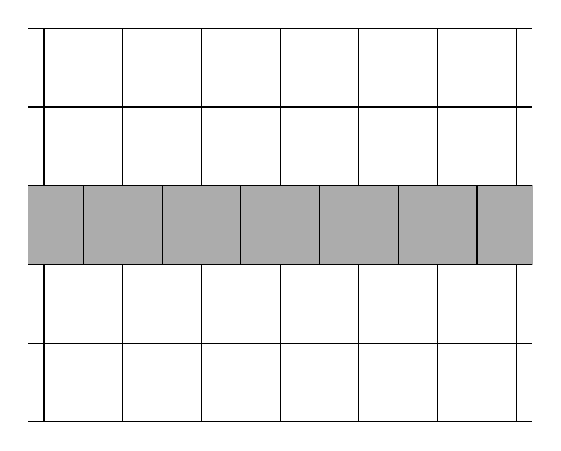
\begin{tikzpicture}[scale=1]
            % Define the tile
            \def\tile{
            \draw[fill=white] (0,0) rectangle (1,1);
            }
            \def\tiletwo{
            \draw[fill=gray!65] (0,0) rectangle (1,1);
            }
            
            % Draw the tiling pattern
            % Everything else
            \foreach \y in {0,1,3,4}{
                \foreach \x in {0,1,2,3,4,5}{
                    \pgfmathsetmacro{\shiftX}{\x} % Set horizontal shift
                    \pgfmathsetmacro{\shiftY}{\y}
                    \begin{scope}[shift={(\shiftX,\shiftY)}]
                        \tile
                    \end{scope}
                }
            }
            % Shifted line
            \foreach \x in {0}{
            \draw[gray!65, fill=gray!65] (\x-0.2,2) rectangle (\x+0.5,3);
            }
            \foreach \x in {6}{
            \draw[gray!65, fill=gray!65] (\x+0.2,2) rectangle (\x-0.5,3);
            }
            % Middle line, must be after the above code in order to get black lines at correct spots
            \foreach \y in {2}{
                \foreach \x in {0,1,2,3,4}{
                    \pgfmathsetmacro{\shiftX}{\x+0.5} % Set horizontal shift
                    \pgfmathsetmacro{\shiftY}{\y}
                    \begin{scope}[shift={(\shiftX,\shiftY)}]
                        \tiletwo
                    \end{scope}
                }
            }
            % small black lines at the top and bottom
            \foreach \y in {0,1,2,3,4,5}{
                \draw (0-0.2,\y) -- (6+0.2,\y);
            }
        \end{tikzpicture}
        %* —————————————————
        \caption{Single row shift}
        \label{fig:single_shift_horizontal_tiling}
    \end{subfigure}\quad
    \begin{subfigure}{.47\textwidth}
        \centering
        %\includegraphics[width=0.9\linewidth]{spec_single_shift.jpg}
        %* Figure 2
        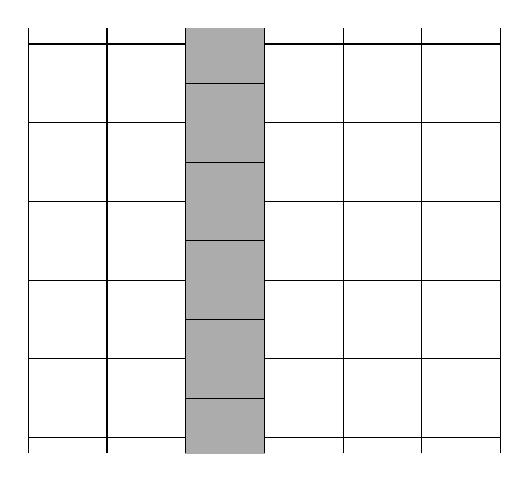
\begin{tikzpicture}[scale=1]
            % Define the tile
            \def\tile{
            \draw[fill=white] (0,0) rectangle (1,1);
            }
            \def\tiletwo{
            \draw[fill=gray!65] (0,0) rectangle (1,1);
            }
            
            % Draw the tiling pattern
            % Everything else
            \foreach \x in {0,1,3,4,5}{
                \foreach \y in {0,1,2,3,4}{
                    \pgfmathsetmacro{\shiftX}{\x} % Set horizontal shift
                    \pgfmathsetmacro{\shiftY}{\y}
                    \begin{scope}[shift={(\shiftX,\shiftY)}]
                        \tile
                    \end{scope}
                }
            }
            % Shifted line
            \foreach \y in {0}{
            \draw[gray!65, fill=gray!65] (2,\y-0.2) rectangle (3,\y+0.5);
            }
            \foreach \y in {5}{
            \draw[gray!65, fill=gray!65] (2,\y+0.2) rectangle (3,\y-0.5);
            }
            % Middle line, must be after the above code in order to get black lines at correct spots
            \foreach \x in {2}{
                \foreach \y in {0,1,2,3}{
                    \pgfmathsetmacro{\shiftX}{\x} % Set horizontal shift
                    \pgfmathsetmacro{\shiftY}{\y+0.5}
                    \begin{scope}[shift={(\shiftX,\shiftY)}]
                        \tiletwo
                    \end{scope}
                }
            }
            % small black lines at the top and bottom
            \foreach \x in {0,1,2,3,4,5,6}{
                \draw (\x,0-0.2) -- (\x,5+0.2);
            }
        \end{tikzpicture}
        %* —————————————————
        \caption{Single column shift}
        \label{fig:single_shift_vertical_tiling}
    \end{subfigure}\\
    \begin{subfigure}{.47\textwidth}
        \centering
        %\includegraphics[width=0.9\linewidth]{multiple_shift_left_zero.jpg}
        %* Figure 3
        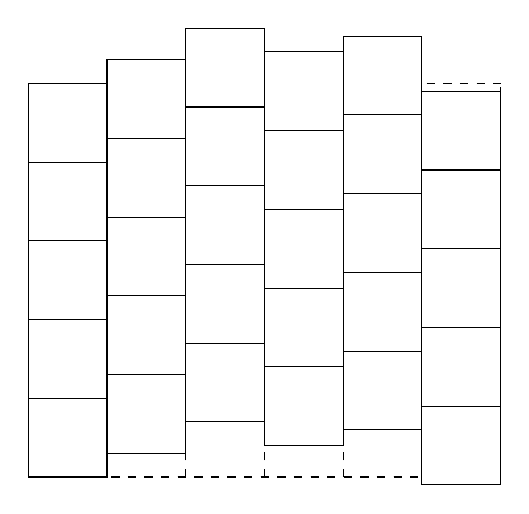
\begin{tikzpicture}[scale=1]
            % Define the tile
            \def\tile{
            % Draw the unit square
            \draw[fill=white] (0,0) rectangle (1,1);
            }

            % Shift list
            \def\BetaMinOne{0}
            \def\BetaZero{0.3}
            \def\BetaOne{0.7}
            \def\BetaTwo{0.4}
            \def\BetaThree{0.6}
            \def\BetaFour{-0.1}
            
            

% Axis lines
%\draw[->] (-1.5,0) -- (4.5,0) node[right] {$X$};
%\draw[->] (0,-1.5) -- (0,3.5) node[above] {$Y$};
\draw[dashed] (0,0) -- (6,0);
\draw[dashed] (0,0) -- (0,5);

% Dashed lines at each integer in the x direction
\foreach \x in {0,...,6}
    \draw[dashed] (\x,0) -- (\x,5);

% Dashed lines at each integer in the y direction
\foreach \y in {0,...,5}
    \draw[dashed] (0,\y) -- (6,\y);


            % Draw the tiling pattern
            \foreach \x in {0,1,2,3,4,5}{
            \foreach \y in {0,1,2,3,4}{
                \ifnum\x=0 % Set vertical shift for the third column only
                    \pgfmathsetmacro{\shiftX}{\x} % No vertical shift for other columns
                    \pgfmathsetmacro{\shiftY}{\y + \BetaMinOne} % Shift one unit upward
                \fi
                \ifnum\x=1
                    \pgfmathsetmacro{\shiftX}{\x}
                    \pgfmathsetmacro{\shiftY}{\y + \BetaZero}
                \fi
                \ifnum\x=2
                    \pgfmathsetmacro{\shiftX}{\x} 
                    \pgfmathsetmacro{\shiftY}{\y + \BetaOne} 
                \fi
                \ifnum\x=3
                    \pgfmathsetmacro{\shiftX}{\x}
                    \pgfmathsetmacro{\shiftY}{\y + \BetaTwo}
                \fi
                \ifnum\x=4
                    \pgfmathsetmacro{\shiftX}{\x}
                    \pgfmathsetmacro{\shiftY}{\y + \BetaThree}
                \fi
                \ifnum\x=5
                    \pgfmathsetmacro{\shiftX}{\x}
                    \pgfmathsetmacro{\shiftY}{\y + \BetaFour}
                \fi
                \begin{scope}[shift={(\shiftX,\shiftY)}]
                \tile % Draw the tile
                \end{scope}
            }}
        \end{tikzpicture}
        %* —————————————————
        \caption{Multiple shifts vertical}
        \label{fig:multiple_shift_vertical_tiling}
    \end{subfigure}\quad
    \begin{subfigure}{.47\textwidth}
        \centering
        %\includegraphics[width=0.9\linewidth]{multiple_shift_left_zero_horizontal.jpg}
        %* Figure 4
        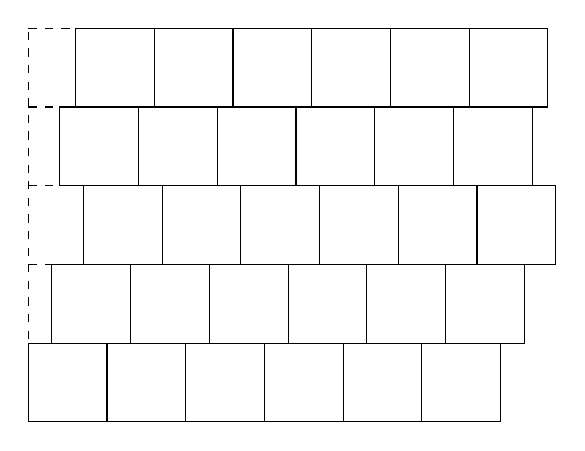
\begin{tikzpicture}[scale=1]
            % Define the tile
            \def\tile{
            % Draw the unit square
            \draw[fill=white] (0,0) rectangle (1,1);
            }

            % Shift list
            \def\BetaMinOne{0}
            \def\BetaZero{0.3}
            \def\BetaOne{0.7}
            \def\BetaTwo{0.4}
            \def\BetaThree{0.6}
            
            

% Axis lines
%\draw[->] (-1.5,0) -- (4.5,0) node[right] {$X$};
%\draw[->] (0,-1.5) -- (0,3.5) node[above] {$Y$};
\draw[dashed] (0,0) -- (6,0);
\draw[dashed] (0,0) -- (0,5);

% Dashed lines at each integer in the x direction
\foreach \x in {0,...,6}
    \draw[dashed] (\x,0) -- (\x,5);

% Dashed lines at each integer in the y direction
\foreach \y in {0,...,5}
    \draw[dashed] (0,\y) -- (6,\y);


            % Draw the tiling pattern
            \foreach \x in {0,1,2,3,4,5}{
            \foreach \y in {0,1,2,3,4}{
                \ifnum\y=0
                    \pgfmathsetmacro{\shiftX}{\x + \BetaMinOne}
                    \pgfmathsetmacro{\shiftY}{\y}
                \fi
                \ifnum\y=1
                    \pgfmathsetmacro{\shiftX}{\x + \BetaZero}
                    \pgfmathsetmacro{\shiftY}{\y}
                \fi
                \ifnum\y=2
                    \pgfmathsetmacro{\shiftX}{\x + \BetaOne} 
                    \pgfmathsetmacro{\shiftY}{\y} 
                \fi
                \ifnum\y=3
                    \pgfmathsetmacro{\shiftX}{\x + \BetaTwo}
                    \pgfmathsetmacro{\shiftY}{\y}
                \fi
                \ifnum\y=4
                    \pgfmathsetmacro{\shiftX}{\x + \BetaThree}
                    \pgfmathsetmacro{\shiftY}{\y}
                \fi
                \begin{scope}[shift={(\shiftX,\shiftY)}]
                \tile % Draw the tile
                \end{scope}
            }}
        \end{tikzpicture}
        %* —————————————————
        \caption{Multiple shifts horizontal}
        \label{fig:multiple_shift_horizontal_tiling}
    \end{subfigure}
    \caption{Text}
    \label{fig:tiling_figures}
\end{figure}



\clearpage
\SigridComment{Gammelt, med gammel struktur}
\begin{definition}[Tiling set]
    Let $\Omega \subset \R^d$ be a subset with nonzero measure, and consider a set $\Lambda \subset \R^d$. If $T(\Lambda)$ cover $\R^d$ up to measure zero, and if all intersections of 
    \begin{equation*}  %* NON OVERLAPPING
        (\Omega+\lambda) \cap (\Omega+\lambda')
    \end{equation*}
    for $\lambda\neq \lambda'$ in $\Lambda$ have measure zero, then $\Omega$ is called a \emph{tile}, and $\Lambda$ is called a \emph{tiling set} for $\Omega$. We say that $(\Omega, \Lambda)$ is a \emph{tiling pair}. 
\end{definition}
\begin{definition}
    Let $\Omega \subset \R^d$ be a subset with nonzero measure, and consider a set $\Lambda \subseteq \R^d$. If the following two conditions are satisfied, then $\Omega$ is called a \emph{tile}, and $\Lambda$ is called a \emph{tiling set} for $\Omega$. We say that $(\Omega, \Lambda)$ is a \emph{tiling pair}. 
    \begin{itemize}
        \item If $T(\Lambda)$ cover $\R^d$ up to measure zero. That is,  %* Cover the whole space
        \begin{equation*}
            \bigcup_{\lambda \in \Lambda} (\Omega + \lambda) = \R^d
        \end{equation*}
        \item If all intersections of $(\Omega+\lambda) \cap (\Omega+\lambda')$ for $\lambda\neq \lambda'$ in $\Lambda$ have measure zero. %* Mutually NON-OVERLAPPING 
    \end{itemize}
\end{definition}


\section{Tiling sets for the n-cube}
\section{The unit cube in dimension one / Tilings in dimension one}
%* Hva vet vi om tilings i en dimensjon for unit cube, jo der har vi bare et alternativ og det er det samme alternativet som for spectral Set
%* paper + andre kilder, søke opp
In dimension one, the unit cube is simply the unit interval $I=\bras{0,1}$.
\begin{theorem}  %* Bruker alle elementene i T for å flytte på I, da dekker vi hele $\R$.  
    Let $\Omega = I$. If $T=\Z$, then $T$ is a tiling set for $I$.
\end{theorem}

\begin{proof}
    It is clear that
    \begin{align*}
        %\bigcup_{\lambda\in \Z} (I + \lambda) &= \bigcup_{\lambda\in \Z} \braq{\omega + \lambda : \omega \in I}\\
        \bigcup_{\lambda\in \Z} (I + \lambda) &= \dots (I-1) \cup (I-0) \cup (I+1) \dots\\ 
        &= \dots [-1,0] \cup [0,1] \cup [1,2] \dots\\
        &= \R
    \end{align*}
    and that 
    \begin{align*}
        \mesMed{\R \setminus \bigcup_{\lambda\in \Z} (I + \lambda) } = \mesMed{\emptyset} = 0.
    \end{align*}
    This shows that the set of translates $T(\Lambda)$ covers $\R$ up to measure zero. 
    
    Now take $\lambda,\lambda' \in \Z$. If $\lambda = \lambda'$ we have that
    \begin{equation*}
        \mes{(I+\lambda) \cap (I+\lambda')} = \mes{(I+\lambda)} = (1+\lambda) - (0+\lambda) = 1.
    \end{equation*}
    And if $\lambda \neq \lambda'$ we have that 
    \begin{equation*}
        \mes{(I+\lambda) \cap (I+\lambda')} = \mes{\emptyset} = 0,
    \end{equation*}
    showing that the cubes are non-overlapping for all distinct $\lambda , \lambda' \in T$. 
\end{proof}


\subsection{The unit cube in higher dimensions / Tilings in higher dimensions}
-> når det er større en 1 har vi flere muligheter

-> en begrensing legges av Kellers theorem, 


\SigridComment{END}



% ! Def tiling
%\begin{definition}[Tiling set]
%    Let $\Omega \subset \mathbb{R}^d$ be a subset with nonzero measure, and consider a set $T \subseteq \mathbb{R}^d$. If the set of translates ${}$$\{\Omega+l: l\in T\}$ cover $\mathbb{R^d}$ up to measure zero, and if all intersections $(\Omega+l) \cap (\Omega+l')$  for $l\neq l'$ in $L$ have measure zero, then $\Omega$ is called a \emph{tile}, and $T$ is called a \emph{tiling set} for $\Omega$. We say that $(\Omega, T)$ is a \emph{tiling pair}. 
%\end{definition}

%In other words, the shifts $\Omega + T$ constitute a \emph{measuredisjoint covering} of $\mathbb{R}^d$, and we can say that $\Omega$ \emph{tiles} $\mathbb{R}^d$ \emph{by translation}, or that $\Omega+T$ is a \emph{tiling} of $\mathbb{R}^d$.


% Fuglede’s spectral set conjecture. Let $\Omega$􏱁 be a set in $\mathbb{R}^d$ with positive and finite Lebesgue measure. Then 􏱁$\Omega$ is a spectral set if and only if $\Omega$􏱁 tiles $\mathbb{R}^d$ by translation.

% An equivalent restatement of Fuglede was presented in Jorgen/Pedersen. 

% Let $\Omega \subset \mathbb{R}^d$ have positive and finite Lebesgue measure. Then $\Omega$ is a spectral set if and only if $\Omega$ is a tile, i.e., there exists a set $\Lambda$ so that $(\Omega, \Lambda)$ is a spectral pair if and only if there exists a set $\Lambda^{\prime}$ so that $\left(\Omega, \Lambda^{\prime}\right)$ is a tiling pair.

%with the following dual conjectures.

% Conjecture 1.3: Let $\Lambda \subset \mathbb{R}^d$. Then $\Lambda$ is a spectrum if and only if $\Lambda$ is a tiling set, i.e., there exists a set $\Omega$ so that $(\Omega, \Lambda)$ is a spectral pair if and only if there exists a set $\Omega^{\prime}$ so that $\left(\Omega^{\prime}, \Lambda\right)$ is a tiling pair.

% Conjecture 1.4: Let $\Lambda \subset \mathbb{R}^d$. Then $\left(I^d, \Lambda\right)$ is a spectral pair if and only if $\left(I^d, \Lambda\right)$ is a tiling pair.

%When  $\Omega = I^d$ the connection between tiles and spectrum is more direct than for other examples of sets $\Omega$. As shown in sigrid_note:lagarias_reeds_wang and Spectral and tiling properties of the unit cube_ALEX IOSEVICH AND STEEN PEDERSEN it is possible to classify all spectra by showing that $\Lambda$ is a spectrum for the unit cube $I^d$, if and only if $I^d$ tiles $\mathbb{R}^d$ by $\Lambda$-translates.






\end{document}


